\section{Hypercubes}
\label{sec:hypercubes}

% One key observation that can be made when looking at the facts of an XBRL report is that they are often structured like a hypercube.
% The aspects of a fact can be seen as the dimensions of a hypercube, whereas the value of the fact is the value of the hypercube at the given dimensions.
% Unlike networks, hypercubes are part of the OIM
% \footnote{Hypercubes are the reason why the OIM does not only cover the XBRL 2.1 core specification, but also the XBRL Dimensions 1.0 specification.}.
A notable insight from examining XBRL report facts is their resemblance to a hypercube structure.
The characteristics of a fact act as the hypercube's dimensions, with the fact's value representing the hypercube's value at those specific dimensions.
Contrary to networks, hypercubes are included within the OIM
\footnote{This inclusion of hypercubes extends the OIM's\cite{oim} scope beyond the XBRL 2.1 core specification\cite{xbrl21} to encompass the XBRL Dimensions 1.0 specification\cite{xbrl_dimensions} as well.}.

% \newfloatcommand{capbtabbox}{table}[][\FBwidth]

% \begin{figure}[H]
%     \caption{Example of a hypercube}
%     % create a figure with side by side images
%     % the first is a table representing a XBRL hypercube.
%     % It has 3 dimensions: "Period", "Entity", and "Concept".
%     % The second image is a 3D representation of the hypercube.
%     \label{fig:example_hypercube}
%     \begin{center}
%         \begin{tabular*}{5cm}{@{\extracolsep{\fill}}|c|c|c|c|}
%             \hline
%             Period & Entity & Concept & Value \\
%             \hline
%             2020 & Foo & Sales & 100\$ \\
%             \hline
%             2020 & Foo & Costs & 50\$ \\
%             \hline
%             2020 & Bar & Sales & 200\$ \\
%             \hline
%             2020 & Bar & Costs & 100\$ \\
%             \hline
%             2021 & Foo & Sales & 150\$ \\
%             \hline
%             2021 & Foo & Costs & 75\$ \\
%             \hline
%             2021 & Bar & Sales & 250\$ \\
%             \hline
%             2021 & Bar & Costs & 125\$ \\
%             \hline
%         \end{tabular*}
%         % TODO: 3D image of hypercube
%         % make it the same height as the table
%         \includegraphics[height=5cm]
%         {images/hypercube_visualization.png}
%     \end{center}
% \end{figure}

\begin{figure}[H]
    \centering
    % 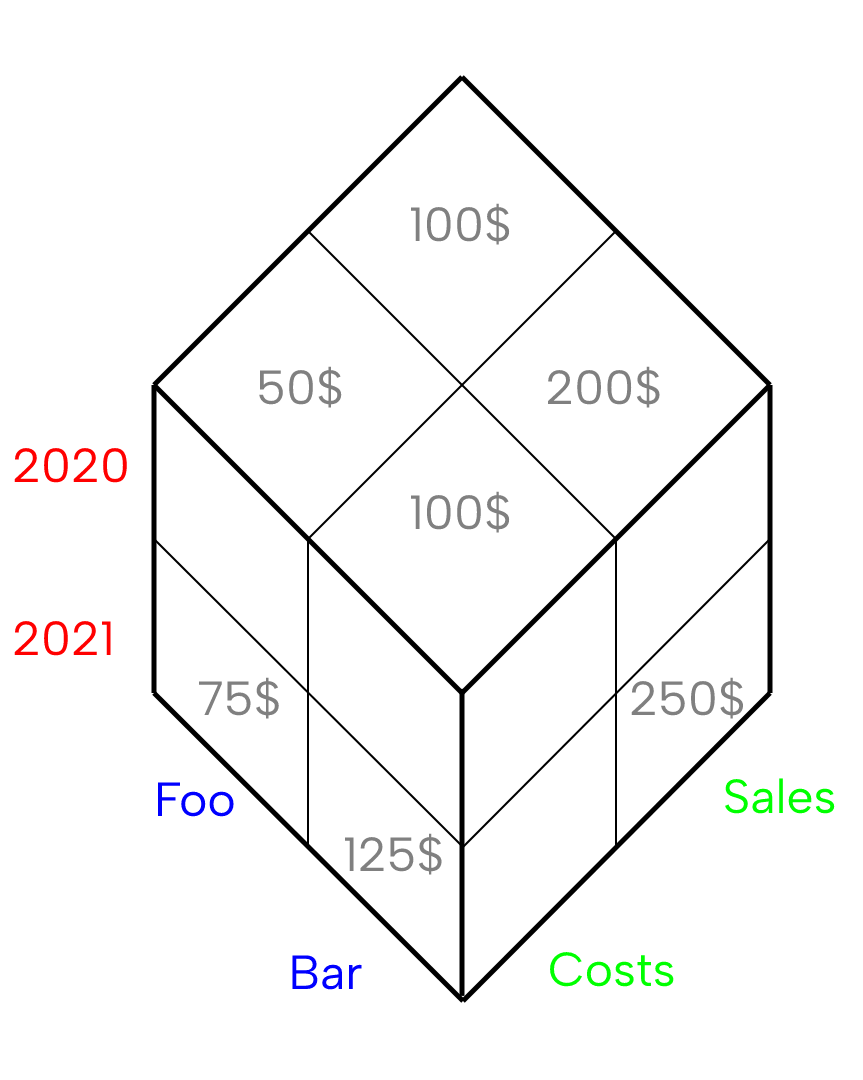
\includegraphics[width=4.6cm]{images/hypercube_visualization.png}
    % \qquad
    \begin{tabular}{|c|c|c|c|}
        \hline
        Period & Entity & Concept & Value \\
        \hline
        2020 & Foo & Sales & \$100 \\
        \hline
        2020 & Foo & Costs & \$50 \\
        \hline
        2020 & Bar & Sales & \$200 \\
        \hline
        2020 & Bar & Costs & \$100 \\
        \hline
        2021 & Foo & Sales & \$150 \\
        \hline
        2021 & Foo & Costs & \$75 \\
        \hline
        2021 & Bar & Sales & \$250 \\
        \hline
        2021 & Bar & Costs & \$125 \\
        \hline
    \end{tabular}
    \caption{Example of a hypercube expressed as a table}
    \label{fig:example_hypercube}
\end{figure}

Figure \ref{fig:example_hypercube} depicts a hypercube with three dimensions: \texttt{Period}, \texttt{Entity}, and \texttt{Concept}.
Each combination of dimensions corresponds to a fact, with the fact's value representing the hypercube's value at those dimensions.

% Hypercubes are a common way to structure data nowadays.
% Yet, back when XBRL was created, they were not as prevalent as they are today.
% In fact, the early versions of XBRL did not support hypercubes at all.
% They were retrofitted into the XBRL specification in 2006.\cite{xbrl_dimensions}.

% \subsection{Dimensions}

% When viewing facts as hypercubes, the cube ends up having four built in dimensions.
% These correspond to the four core aspects of a fact: \texttt{Period}, \texttt{Entity}, \texttt{Concept}, and \texttt{Unit}.
% XBRL allows for the creation of custom dimensions, which come in two flavors: explicit and typed.

% Unfortunately, XBRL overloads the term "dimension".
% It refers to both the dimensions of a hypercube, as well as the two custom dimension types. 

% \subsection{Explicit dimensions}

% Explicit dimensions are dimensions that have a predefined set of possible values.
% For example, let us assume that the Foo Company has two subsidiaries: Foo United States and Foo Europe.
% The Foo Company could then create a dimension called \texttt{Subsidiary} with the two possible values \texttt{Foo United States} and \texttt{Foo Europe}.
% The possible values of an explicit dimension are called \texttt{members}.

% Both dimensions and members are defined using report elements, just like concepts and abstracts before them.
% To symbolize that a member belongs to a dimension, the member is defined as a child of the dimension in the definition network.

% The members of a dimension can also have even more child members themselves.
% For example, the Subsidiary Foo Europe could have two subsidiaries: Foo Switzerland and Foo EU.

Data structuring through hypercubes has become widely adopted in recent times.
However, when XBRL was initially developed, hypercubes were not as commonly used.
The early versions of XBRL lacked hypercube support,
which was later integrated into the XBRL framework in 2006.\cite{xbrl_dimensions}.

\subsection{Dimensions}

Considering facts as components of a hypercube introduces four inherent dimensions.
These dimensions align with the primary aspects of a fact: \texttt{Period}, \texttt{Entity}, \texttt{Concept}, and \texttt{Unit}.
XBRL facilitates adding custom dimensions, categorized as either explicit or typed.

The terminology "dimension" is used in XBRL to denote both the hypercube's dimensions and the two types of custom dimensions.

\subsection{Explicit dimensions}

Explicit dimensions specify dimensions with a set range of possible values.
For instance, consider the Foo Company operates two branches: Foo United States and Foo Europe.
The company could establish a \texttt{Subsidiary} dimension featuring \texttt{Foo United States} and \texttt{Foo Europe} as possible values.
These predefined values are referred to as \texttt{members}.

Both \texttt{dimensions} and \texttt{members} are designated through report elements, akin to concepts and abstracts.
A member is depicted as part of a dimension by positioning it as a dimension's child within the definition network.

Moreover, members within a dimension may possess their own subordinate members.
As an illustration, Foo Europe could encompass two subsidiaries: Foo Switzerland and Foo EU.

\begin{figure}[H]
    \label{fig:example_explicit_dimension}
    \caption{Visualizations of the explicit dimension "Subsidiary"}
    \dirtree{%
        .1 [Dimension] Subsidiary.
        .2 [Member] Foo United States.
        .2 [Member] Foo Europe.
        .3 [Member] Foo Switzerland.
        .3 [Member] Foo EU.
    }
\end{figure}

% \subsection{Typed dimensions}

% Typed dimensions are dimensions that do not have a predefined set of possible values.
% Instead, the values of a typed dimension are constrained by a data type.
% For example, a dimension could be constrained to only allow values of the type \texttt{xs:integer}.

% Similar to explicit dimensions, typed dimensions are defined using report elements.
% Unlike explicit dimensions, typed dimensions do not have members.
% They consist solely of the dimension report element, which defines the data type of the dimension.

% \subsection{Line items and hypercubes}

% With our current understanding of hypercubes, we can only view the whole report as a single, gigantic hypercube.
% Especially when considering the additional dimensions, most facts will use only a small subset of the possible dimensions.
% This makes the resulting hypercube high dimensional, with most of the dimensions being unused.
% Using the large hypercube as a basis for analysis would be very inefficient.

% To solve this problem, XBRL introduces the \texttt{hypercube} report element.
% Conceptually, a hypercube is a sub-hypercube of the whole report hypercube.
% Hypercube report elements are usually defined an a per-role basis as part of a definition network.
% It picks a subset of the dimensions of the whole report hypercube.
% This subset is determined in the definition network, where "hypercube-dimension" arcs specify which dimensions are part of the hypercube.

% Besides the hypercube report element, XBRL also introduces the \texttt{lineItems} report element.
% LineItems are used to specify which concepts are part of the hypercube.
% Reports can specify tens of thousands of concepts, but only a few of them are relevant for a particular role.
% The LineItems report element specifies the relevant concepts by listing them as children in the definition network.

% If understanding lineItems proves to be difficult, consider the following: 
% LineItems are to concepts what dimensions are to members.

\subsection{Typed dimensions}

Typed dimensions differ from explicit dimensions by not having a pre-established set of possible values.
Instead, the scope of values for a typed dimension is defined by a specific data type.
For instance, a dimension may be restricted to accept only \texttt{xs:integer} type values.

Just like explicit dimensions, typed dimensions are also delineated through report elements.
However, unlike explicit dimensions, typed dimensions do not include members but consist only of the dimension report element, which contains the dimension's data type.

\subsection{Line Items and Hypercubes}

Given our understanding of hypercubes, it's apparent that the entire report could be viewed as a large hypercube.
Particularly with the addition of extra dimensions, it's likely that most facts will use just a fraction of the available dimensions.
This scenario results in a highly dimensional hypercube, with many dimensions remaining unutilized.
Analyzing the report based on this large hypercube would be inefficient.

XBRL addresses this issue by introducing the \texttt{hypercube} report element.
A hypercube is conceptually a smaller sub-cube of the overarching report hypercube.
Hypercube report elements are typically defined on a role-specific basis within a definition network.
They select a subset of the dimensions from the entire report hypercube,
determined within the definition network, where “hypercube-dimension” arcs indicate the included dimensions.

XBRL further introduces the \texttt{lineItems} report element.
Line items pinpoint which concepts belong to the hypercube.
Although a report might detail tens of thousands of concepts, only a select number are relevant for a given role.
The line items report element identifies these relevant concepts by listing them as children within the definition network.

% For a clearer understanding, think of lineItems in relation to concepts as dimensions are related to members.
The reader may think of the relationship between line items and concepts as akin to that between dimensions and members.

% \subsection{Open Hypercubes}

% % So far, we have only considered hypercubes that are fully defined.
% Up to this point, we have only examined fully defined hypercubes.
% Each member of each dimension is a known report element defined in the taxonomy.
% % This is known as a closed hypercube.
% This is referred to as a closed hypercube.

% % However, XBRL also supports open hypercubes.
% However, XBRL also accommodates open hypercubes, 
% % Open hypercubes are hypercubes that have dimensions with members that are not known in advance.
% which are hypercubes featuring dimensions with members that are not predefined.
% % So the hypercubes might reference members that are not defined in the taxonomy.
% Consequently, the hypercube may reference members that are not defined in the taxonomy.

% % The current implementation of Brel does not support open hypercubes, but it is a feature that is planned for the future.
% Currently, Brel does not support open hypercubes, but this feature is planned for future implementation.
% % Section \ref{sec:implementation} will cover why open hypercubes are not supported for now.
% The reasons for the lack of support for open hypercubes will be detailed in section \ref{sec:implementation}.
